\documentclass[sigconf,authordraft]{acmart}

\usepackage{gensymb}
\usepackage[inline]{enumitem}

\AtBeginDocument{%
  \providecommand\BibTeX{{%
    \normalfont B\kern-0.5em{\scshape i\kern-0.25em b}\kern-0.8em\TeX}}}

\citestyle{acmauthoryear}

\begin{document}

\title{Application of Reinforcement Learning in NASA Swarmathon Competition}

\author{Rolando J. Nieves}
\email{rolando.j.nieves@knights.ucf.edu}
\authornotemark[1]
\affiliation{%
  \institution{University of Central Florida}
  \streetaddress{4000 Central Florida Blvd.}
  \city{Orlando}
  \state{Florida}
  \postcode{32816}
}

\renewcommand{\shortauthors}{Nieves}

\begin{abstract}
  The NASA Swarmathon competition domain provides an excellent proving ground
  for the implementation of multi-agent cooperative behavior using Reinforcement
  Learning (RL). This report documents the results of a study aimed at replacing
  the fixed, swarm-like logic offered as a baseline to competition entrants with
  a system that can be trained in a simulated environment prior to deployment
  onto an entrant's physical robots.
\end{abstract}

\begin{CCSXML}
  <ccs2012>
    <concept>
      <concept_id>10010147.10010178.10010219.10010220</concept_id>
      <concept_desc>Computing methodologies~Multi-agent systems</concept_desc>
      <concept_significance>500</concept_significance>
    </concept>
    <concept>
      <concept_id>10010147.10010257.10010258.10010261.10010275</concept_id>
      <concept_desc>
        Computing methodologies~Multi-agent reinforcement learning
      </concept_desc>
      <concept_significance>500</concept_significance>
    </concept>
  </ccs2012>
\end{CCSXML}

\ccsdesc[500]{Computing methodologies~Multi-agent systems}
\ccsdesc[500]{Computing methodologies~Multi-agent reinforcement learning}

\keywords{multi-agent systems,machine learning,reinforcement learning}

\begin{teaserfigure}
  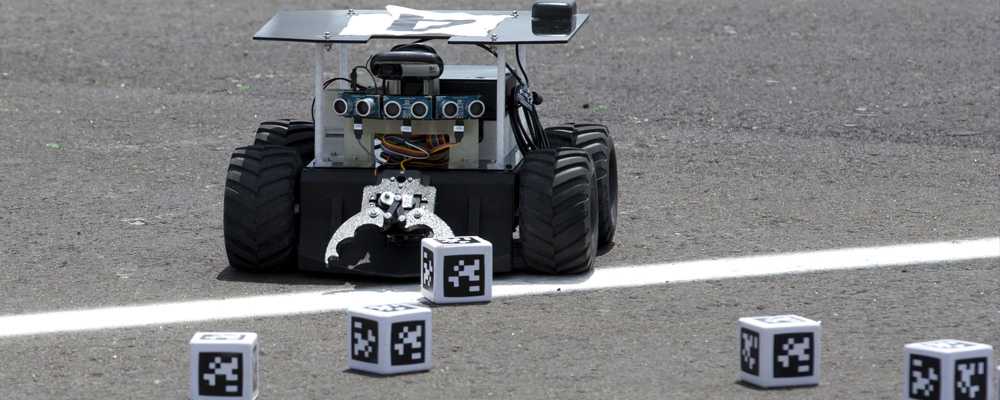
\includegraphics[width=\textwidth]{images/swarmathon-teaser.jpg}
  \caption{Montgomery College ``Swarmie'' in 2017 NASA Swarmathon}
  \Description{Image of a robotic member of the Montgomery College Swarmathon team entrant competing in NASA Swarmathon 2017}
  \label{fig:teaser}
\end{teaserfigure}

\maketitle

\section{Introduction}\label{sec:intro}
The study of applying Reinforcement Learning (RL) into cooperative multi-agent
systems remains a hot topic at the time of this writing. The topic's popularity
owes primarily to the fact that, unlike single agent RL, no single system
architecture has yet emerged as clearly superior among all available options.
Current architectural patterns such as Independent Learners (IL) and
Joint-Action Learners (JAL) exhibit traits that in some environments prove
quite beneficial. In other environments, however, these same traits represent
intolerable liabilities.

Thus, the search for a ``better mouse trap'' in the area of cooperating,
multi-agent RL has led to a proliferation of problem domains under which
methodology performance can be tested and quantified. From grid-world like
synthetic predator-prey scenarios, to more flexible environments like RoboCup
Simulated Soccer, these domains offer efficient ways to test theories. One
shortcoming of these problem domains, however, is the difficulty of implementing
any realized achievements into a physical domain.

The NASA Swarmathon problem domain offers an exciting opportunity for research
in this field. This is so because, combined with a robust simulation environment
based around the Robot Operating System (ROS) software suite, the domain offers
a clear path to implementation into physical robots participating in live
competition.

\section{Problem Domain}\label{sec:prob_domain}
In a generic sense, NASA Swarmathon is a resource gathering exercise using a
swarm of autonomous robots. The robotic swarm is expected to gather a set of
resources from their surrounding environment onto a collection area without
relying on any human supervision. NASA's intent with the competition is the
development of technologies that could one day be used to deploy ``advance
missions'' that perform as much preparation as possible at a planetary body site ahead of the arrival by human explorers.

NASA defines the Swarmathon competition environment using the following
elements:

\begin{itemize}
  \item A $16 \times 16$ or $32 \times 32$ meter square field where the
  competition takes place. The field size varies based on the round the
  competition is at.
  \item A swarm of three or six robots, with each robot labeled as a
  ``swarmie.''
  \item Up to 256, $2 \times 2 \times 2$ inch cubes bearing ``April Tag''
  markers on all six faces, known as ``April Cubes.''
  \item A $1 \times 1$ meter square collection area within the competition
  field, known as a ``nest.''
\end{itemize}

During a competition round, a set of ``April Cubes'' are randomly strewn across
open areas of the competition field (i.e., no cubes initially start at
the ``nest''). The robotic swarm is then tasked with collecting the cubes onto
the ``nest.'' The periphery of the nest is labeled using another set of ``April
Tags,'' serving as a visual indicator for the robots. Collected cubes must be
in contact with the ``nest'' in order for them to count towards the team's
overall score.

Team members are not allowed contact or communication with the robots
(``swarmies'') during a round, leaving the robots to complete the task
leveraging their built-in sensor package and logic deployed to them prior to the
round. Individual robots are, however, allowed to communicate amongst
themselves. Although no restrictions on underlying physical communication fabric
exists as of this writing, the selected physical fabric must be exposed to the
robots via the ROS Publish-Subscribe communication system. A popular choice among teams is the use of Wi-Fi networking to implement robot-to-robot communication. No restrictions regarding bandwidth or reliability is imposed on the teams as of this writing.

The elements that comprise the ``swarmie'' sensor package include the
following:

\begin{itemize}
  \item Three ultrasonic range finders able to detect obstacles up to 3 meters
  away. The sensors are located in front of the robot, and evenly distributed
  across a $60^{\circ}$ arc.
  \item One Inertial Measurement Unit (IMU) used to estimate robot orientation
  and, in combination with other sensors, robot pose in the fixed competition
  area.
  \item One camera emitting color $320 \times 240$ resolution images at about
  six frames per second (FPS).
  \item One Global Positioning Satellite (GPS) receiver emitting latitude and
  longitude readings that, in combination with other sensors, help establish the
  robot's pose in the competition area.
  \item One odometer emitting wheel movement that, in combination with other
  sensors, help establish the robot's pose in the competition area.
\end{itemize}

In order to combine, or ``fuse,'' several of the sensor readings into a complete
robot pose, the baseline software provided by NASA includes an Extended Kalman
Filter (EKF) pipeline that eventually produces the following pose information:

\begin{itemize}
  \item Cartesian $(x,y,z)$ position with (albeit mostly static) altitude.
  \item Yaw with respect to a fixed reference frame.
  \item Linear $(x,y)$ velocity.
  \item Angular velocity about the Yaw axis
  \item Linear $(x,y)$ acceleration. 
\end{itemize}

Given that the robots are four-wheeled traversing a flat area, linear velocity
and acceleration in the altitude $z$ axis, as well as angular position and
velocity about the Roll and Pitch axes is not calculated.

The NASA baseline software also includes computer vision facilities that, when
combined with the camera and robot pose calculations, are able to provide
information about any ``April Tags'' visible within the robot's field of view.
As stated previously, the ``April Cubes'' that the robots must gather are
labeled on all six faces with the aforementioned tags, as is the ``nest''
periphery where the robots must deposit the cubes.

The NASA baseline software is written in terms of the facilities and services
provided by ROS, particularly when it comes to communication. Software provided
by teams must run within ROS and, again, may only utilize the Publish-Subscribe
system provided with ROS for their communication needs. In addition, the NASA
baseline software provides a simulation environment that combines ROS Gazebo
with 3D models of the robots and sensor emulation. During a simulation session,
the communication traffic fed as input to the software components that combine
to implement a robot's logic is practically indistinguishable from traffic that
would be produced by the sensor package of a physical robot.

\section{Related Works}\label{sec:related_works}
Related works discussion.

\section{Methodology}\label{sec:methodology}
There are many aspects of the NASA Swarmathon domain that pose a challenge against the implementation of a Reinforcement Learning (RL) based solution. Chief among these challenges are:

\begin{itemize}
  \item Although the number of ``April Cubes'' the Swarmies are tasked with foraging is fixed and known, their exact location in the arena is not.
  \item The Swarmies identify the location of ``April Cubes'' using two-dimensional cartesian coordinates $\textbf{L} \in \mathbb{R}^2$ based on the coordinate reference frame individually maintained by each Swarmie.
  \item The Swarmies navigate the competition area primarily using waypoints that are specified as two-dimensional cartesian coordinates $\textbf{W} \in \mathbb{R}^2$, again based on the individual reference frame maintained by each Swarmie.
  \item The Swarmies are not designed to properly map the competition area, thus they are required to continuously detect and properly react to the area's boundaries as well as the collection ``nest.''
\end{itemize}

Addressing each one of the aforementioned challenges is not impossible, but does impact the RL-based solution in ways that could introduce some margin of error and uncertainty.

The lack of persistent mapping capability by the Swarmies is not too difficult a challenge, as both the robot's sensor package and competition area markings make it possible to navigate without having to resort to a map or known landmark locations. The baseline NASA Swarmathon software code contains low-level logic that enables
\begin{enumerate*}[label={(\arabic*)}]
  \item the detection and avoidance of physical obstacles,
  \item the detection of the collection zone (i.e., the ``nest''), and
  \item the detection and avoidance of the competition area boundary.
\end{enumerate*}
Thus, given that hazard avoidance is not the main focus of this RL-based solution, integrating the existing logic is the most efficient course of action to address the challenge.

Considered in isolation, the requirement that the robotic swarm find the location of all the ``April Cubes'' with very little prior knowledge is not a very difficult problem. Indeed, such a problem closely resembles a run-of-the-mill mapping exercise. The complications begin to arise once the following facts are taken into consideration:

\begin{itemize}
  \item Each Swarmie calls out the location of each ``April Cube'' observed in the competition area using real-space coordinates based on the robot's individual reference frame.
  \item The reference frame maintained by each Swarmie centers its origin at the robot's starting location.
  \item Even with sensor fusion, the reported location by each Swarmie varies by as much as $\pm 0.5$ meters with each sensor reading.
\end{itemize}

The presence of multiple reference frames can be addressed via the use of a simple affine transform to a global reference frame. Given that, at the start of a simulated run, the location of each Swarmie is specified in such a global reference frame, the parameters for such a transform (which would only include a translation component) can be easily communicated to each robot.

The use of real-space coordinates, combined with the variability introduced by the sensor package, makes it nearly impossible to properly attach a true location for an individual ``April Cube,'' even after applying a global reference frame transform. Although a system could be devised that could combine multiple observations with SLAM-like techniques to narrow the sensor variability, such is not the focus of this study.

Instead, a more economical approach involves the discretization of the competition area, making it resemble a ``grid world,'' at least for the purposes of ``April Cube'' mapping. Given the perceived position variability, at least as produced by sensor fusion, a good starting point for a grid world cell size could be $0.5 \times 0.5$ meters square. Making the grid world cell size into a hyper-parameter of the model makes it possible to supplement the optimization options of the resulting system.

Since in almost all cases the grid world cell size will be far larger than the surface area occupied by an individual ``April Cube,'' there exists a very good possibility that multiple cubes will occupy a particular cell. Thus, even after discretization, uniquely attaching a location for each cube remains elusive. However, given that the total number of cubes present is known to each robot, it is possible to indirectly attach a state label to the cubes present in the competition area. Consider that, at any one time, ``April Cube'' subsets could be incorporated into one of four mutually-exclusive states:

\begin{description}
  \item[At-Large]: Cubes that are known to exist, but whose location remains unknown.
  \item[Located]: Cubes that are known to be occupying a cell in the competition area grid world, outside of the collection zone.
  \item[In-Transit]: Cubes being transported by Swarmie robots to the collection zone.
  \item[Collected]: Cubes known to be present in the collection zone.
\end{description}

Given that the subsets are mutually exclusive, a simple mathematical relation can be drawn from their individual membership sizes. Let $N$ be the total number of cubes known to exist, $B_u$ be the number cubes considered \textbf{At-Large}, $B_l$ be the number of cubes considered \textbf{Located}, $B_t$ be the number of cubes considered \textbf{In-Transit}, and $B_c$ be the number of cubes considered \textbf{Collected}. Equation \ref{eq:cube_count_relation} depicts the mathematical relation.

\begin{equation}\label{eq:cube_count_relation}
  N = B_u + B_l + B_t + B_c
\end{equation}

The count of ``April Cubes'' considered \textbf{In-Transit} or \textbf{Collected} is pretty self-explanatory. The count of cubes considered \textbf{Located} ($B_l$) is a little more nebulous. Given the conditions that led to the discretization of the competition area, not every individual cube spotted by a Swarmie robot will be immediately accounted for in $B_l$. A more apt description for the set would be the number of competition area grid cells known to be occupied by at least one ``April Cube.'' Thus, during most of the competition run, $B_l$ will under-estimate the number of cubes spotted by Swarmies. Fortunately, the combination of the known total cube count ($N$), Equation \ref{eq:cube_count_relation}, and the \textbf{At-Large} set size ($B_u$) help to ensure that any located cube under-count is eventually rectified. Once a grid world cell is considered ``unoccupied'' (e.g., due to a cube in the cell being picked up), the spotting of another cube in the same cell will transition a cube from \textbf{At-Large} to \textbf{Located} (i.e., bump $B_l$ at the expense of $B_u$). Such transitions help lift the ``fog of war'' that obfuscates the location of ``April Cubes,'' manifested by the $B_u$ term in Equation \ref{eq:cube_count_relation}.

The set counts in Equation \ref{eq:cube_count_relation} serve as an excellent starting point for defining the state space that the Reinforcement Learning algorithm in this Swarmathon solution uses.

\section{Experimental Results}\label{sec:results}
Results discussion.

\section{Conclusion}\label{sec:conclusion}
Final conclusion.

\bibliographystyle{ACM-Reference-Format}
\bibliography{swarmies_rl}

\end{document}
